% Options for packages loaded elsewhere
\PassOptionsToPackage{unicode}{hyperref}
\PassOptionsToPackage{hyphens}{url}
%
\documentclass[
  12pt,
  landscape]{article}
\usepackage{lmodern}
\usepackage{amssymb,amsmath}
\usepackage{ifxetex,ifluatex}
\ifnum 0\ifxetex 1\fi\ifluatex 1\fi=0 % if pdftex
  \usepackage[T1]{fontenc}
  \usepackage[utf8]{inputenc}
  \usepackage{textcomp} % provide euro and other symbols
\else % if luatex or xetex
  \usepackage{unicode-math}
  \defaultfontfeatures{Scale=MatchLowercase}
  \defaultfontfeatures[\rmfamily]{Ligatures=TeX,Scale=1}
\fi
% Use upquote if available, for straight quotes in verbatim environments
\IfFileExists{upquote.sty}{\usepackage{upquote}}{}
\IfFileExists{microtype.sty}{% use microtype if available
  \usepackage[]{microtype}
  \UseMicrotypeSet[protrusion]{basicmath} % disable protrusion for tt fonts
}{}
\makeatletter
\@ifundefined{KOMAClassName}{% if non-KOMA class
  \IfFileExists{parskip.sty}{%
    \usepackage{parskip}
  }{% else
    \setlength{\parindent}{0pt}
    \setlength{\parskip}{6pt plus 2pt minus 1pt}}
}{% if KOMA class
  \KOMAoptions{parskip=half}}
\makeatother
\usepackage{xcolor}
\IfFileExists{xurl.sty}{\usepackage{xurl}}{} % add URL line breaks if available
\IfFileExists{bookmark.sty}{\usepackage{bookmark}}{\usepackage{hyperref}}
\hypersetup{
  pdftitle={Applications of Econometrics and Data Science Methods Pset1},
  pdfauthor={Jack Ogle and Izzy Allum},
  hidelinks,
  pdfcreator={LaTeX via pandoc}}
\urlstyle{same} % disable monospaced font for URLs
\usepackage[margin=1in]{geometry}
\usepackage{color}
\usepackage{fancyvrb}
\newcommand{\VerbBar}{|}
\newcommand{\VERB}{\Verb[commandchars=\\\{\}]}
\DefineVerbatimEnvironment{Highlighting}{Verbatim}{commandchars=\\\{\}}
% Add ',fontsize=\small' for more characters per line
\usepackage{framed}
\definecolor{shadecolor}{RGB}{248,248,248}
\newenvironment{Shaded}{\begin{snugshade}}{\end{snugshade}}
\newcommand{\AlertTok}[1]{\textcolor[rgb]{0.94,0.16,0.16}{#1}}
\newcommand{\AnnotationTok}[1]{\textcolor[rgb]{0.56,0.35,0.01}{\textbf{\textit{#1}}}}
\newcommand{\AttributeTok}[1]{\textcolor[rgb]{0.77,0.63,0.00}{#1}}
\newcommand{\BaseNTok}[1]{\textcolor[rgb]{0.00,0.00,0.81}{#1}}
\newcommand{\BuiltInTok}[1]{#1}
\newcommand{\CharTok}[1]{\textcolor[rgb]{0.31,0.60,0.02}{#1}}
\newcommand{\CommentTok}[1]{\textcolor[rgb]{0.56,0.35,0.01}{\textit{#1}}}
\newcommand{\CommentVarTok}[1]{\textcolor[rgb]{0.56,0.35,0.01}{\textbf{\textit{#1}}}}
\newcommand{\ConstantTok}[1]{\textcolor[rgb]{0.00,0.00,0.00}{#1}}
\newcommand{\ControlFlowTok}[1]{\textcolor[rgb]{0.13,0.29,0.53}{\textbf{#1}}}
\newcommand{\DataTypeTok}[1]{\textcolor[rgb]{0.13,0.29,0.53}{#1}}
\newcommand{\DecValTok}[1]{\textcolor[rgb]{0.00,0.00,0.81}{#1}}
\newcommand{\DocumentationTok}[1]{\textcolor[rgb]{0.56,0.35,0.01}{\textbf{\textit{#1}}}}
\newcommand{\ErrorTok}[1]{\textcolor[rgb]{0.64,0.00,0.00}{\textbf{#1}}}
\newcommand{\ExtensionTok}[1]{#1}
\newcommand{\FloatTok}[1]{\textcolor[rgb]{0.00,0.00,0.81}{#1}}
\newcommand{\FunctionTok}[1]{\textcolor[rgb]{0.00,0.00,0.00}{#1}}
\newcommand{\ImportTok}[1]{#1}
\newcommand{\InformationTok}[1]{\textcolor[rgb]{0.56,0.35,0.01}{\textbf{\textit{#1}}}}
\newcommand{\KeywordTok}[1]{\textcolor[rgb]{0.13,0.29,0.53}{\textbf{#1}}}
\newcommand{\NormalTok}[1]{#1}
\newcommand{\OperatorTok}[1]{\textcolor[rgb]{0.81,0.36,0.00}{\textbf{#1}}}
\newcommand{\OtherTok}[1]{\textcolor[rgb]{0.56,0.35,0.01}{#1}}
\newcommand{\PreprocessorTok}[1]{\textcolor[rgb]{0.56,0.35,0.01}{\textit{#1}}}
\newcommand{\RegionMarkerTok}[1]{#1}
\newcommand{\SpecialCharTok}[1]{\textcolor[rgb]{0.00,0.00,0.00}{#1}}
\newcommand{\SpecialStringTok}[1]{\textcolor[rgb]{0.31,0.60,0.02}{#1}}
\newcommand{\StringTok}[1]{\textcolor[rgb]{0.31,0.60,0.02}{#1}}
\newcommand{\VariableTok}[1]{\textcolor[rgb]{0.00,0.00,0.00}{#1}}
\newcommand{\VerbatimStringTok}[1]{\textcolor[rgb]{0.31,0.60,0.02}{#1}}
\newcommand{\WarningTok}[1]{\textcolor[rgb]{0.56,0.35,0.01}{\textbf{\textit{#1}}}}
\usepackage{graphicx,grffile}
\makeatletter
\def\maxwidth{\ifdim\Gin@nat@width>\linewidth\linewidth\else\Gin@nat@width\fi}
\def\maxheight{\ifdim\Gin@nat@height>\textheight\textheight\else\Gin@nat@height\fi}
\makeatother
% Scale images if necessary, so that they will not overflow the page
% margins by default, and it is still possible to overwrite the defaults
% using explicit options in \includegraphics[width, height, ...]{}
\setkeys{Gin}{width=\maxwidth,height=\maxheight,keepaspectratio}
% Set default figure placement to htbp
\makeatletter
\def\fps@figure{htbp}
\makeatother
\setlength{\emergencystretch}{3em} % prevent overfull lines
\providecommand{\tightlist}{%
  \setlength{\itemsep}{0pt}\setlength{\parskip}{0pt}}
\setcounter{secnumdepth}{-\maxdimen} % remove section numbering
\usepackage{dcolumn}
\usepackage{float}
\usepackage{graphicx}
\usepackage{amsmath}

\title{Applications of Econometrics and Data Science Methods Pset1}
\author{Jack Ogle and Izzy Allum}
\date{}

\begin{document}
\maketitle

Problem 1 (a)

Propose a sequence of random variables that converges in probability to
p.~This sequence must be a function that maps sample sizes (i.e.~natural
numbers) to random variables. Hint: Recall the weak law of large
numbers.

From the Law of Large numbers and the Central Limit Theorem we know that
a sequence of random variables \({\theta_N }\) converges in probability
to \({\theta}\) if for any \({\epsilon} > 0\) and \({\delta} > 0\) there
exists \({N^*} = N^*(\epsilon, \delta)\) such that for all \({N > N^*}\)

Where \(\theta_N\) is a function of \((y_i, X_i, i = 1,...N)\)

\[
Pr(|\theta_N-\theta|<\epsilon) >1-\delta
\] If the limit exists we write that \({\theta_N}\) converges in
probability to \(\theta\). And because p is the percentage of COVID-19
infected in Chicago we also know that it has a Bernoulli distribution.
Our end goal is to estimate the number of total test kits needed for the
entire population of Chicago. Therefore we want to estimate the
postitivity rate of Chicago. We can't observe the entire population, but
we can observe a sample. We use the sample to estimate p and we know
that through the law of large numbers and the central limit theorem if
you substitute \(\theta\) for p.~Our sample \(Pn\) will converge in
probability to \(P\).

\begin{enumerate}
\def\labelenumi{(\alph{enumi})}
\setcounter{enumi}{1}
\item
\end{enumerate}

The classical Central Limit Theorem assumptions are that:

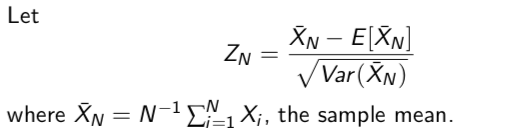
\includegraphics{/users/matthewogle/ds-metrics/pset1/let.png}

\begin{enumerate}
\def\labelenumi{(\roman{enumi})}
\tightlist
\item
  Let \(X_i\) be iid with \(E[X_i] = \mu\)
\end{enumerate}

Since all \(X_i\) are Bernoulli and mutually independent this condition
is satisfied.

\begin{enumerate}
\def\labelenumi{(\roman{enumi})}
\setcounter{enumi}{1}
\item
  and \(Var(X_i) = \sigma^2\) meaning that our variance is finite. Then
  \(Z_N\) in distribution to a normal distribution of N(0,1). And
  because our \(Var(X_i) = p(1-p)\) our variance.
\item
\end{enumerate}

With the Central Limit Theorem even though the population of Chicago
might not be normal we can extend the Single Sample Hypothesis test for
normally distributed populations to those that are not normally
distributed. We have a sample of size n, where n is sufficiently large.
The null hypothesis is: \(H_0: p = p_0\).

The alternative hypothesis is \(H_1: p > p_0\)

When we assume the null hypothesis, we know from CLT that the sample
mean has a normal distribution.

We will assume that the level of significance is \(\alpha\). Because our
sample takes on a bernoulli distribution we know that \(X_N\)
\textasciitilde{} Binomial (p, \(\frac{p(1-p)}n\))

From b) we know that our variables and sample satisfy CLT assumptions
and can therefore conclude that our
\[\frac{X_N-p}{\sqrt{\frac{p(1-p)}{n}}}\] converges in distribution to a
standard normal distribution N(0,1).

Now lets evaluate our null hypotheses \(H_0\) which states that
\[\frac{X_N-p_0}{\sqrt{\frac{p_0(1-p_)}{n}}}\] converges in distribution
to a standard normal distribution N(0,1).

Because the alternative hypothesis contains an greater than inequality
we will use a right hand test. To find the critical value we must find
the region that is greater than \(Z_{1-\alpha}\). The rejection region
is

\[
Z_{1-\alpha} < \frac{X_N-p_0}{\sqrt{\frac{p_0(1-p_)}{n}}}
\] - this is our test statistic.

Solving for our sample mean. Our official rejection region is:

\[
X_n > \frac{Z_{1-\alpha} \sqrt{p_0(1 - p_0)}} {\sqrt{n}} + p_0 
\]

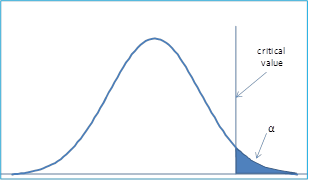
\includegraphics{/users/matthewogle/ds-metrics/pset1/righthand.png}

\begin{enumerate}
\def\labelenumi{(\alph{enumi})}
\setcounter{enumi}{3}
\tightlist
\item
  Without the asymptomatic results we cannot use CLT. We must use the
  fact that our sample has a bernoulli distribution. This means that
  \({X_n}\) are binomial like we established in c). \(X_N\)
  \textasciitilde{} Binomial (p, \(\frac{p(1-p)}{n}\))
\end{enumerate}

We reject the null hypothesis when \(X_n > C_b\) assuming that the
following condition is met:

\[
\sum_{k = c_b}^{n}\begin{pmatrix} n \\ k \end{pmatrix}p_0^k
(1-p_0)^{n-k} \leq \alpha
\]

\begin{enumerate}
\def\labelenumi{(\alph{enumi})}
\setcounter{enumi}{4}
\item
\end{enumerate}

In this question we need to solve for the number of test kits here. In
order to do that we need to find an n (number of test kits) such that
the critical value for the type I and the type II errors are equal to
each other. The type I errors are those that fall under \(H_0\) and the
type II errors are those that fall under \(H_1\)

\[
\frac{Z_{1 - \alpha}\sqrt{p_0(1-p_0)}} {\sqrt{n}} + p_0 
\] =

\[
\frac{Z_{1 - \alpha}\sqrt{p_1(1-p_1)}} {\sqrt{n}} + p_1 
\]

Now we solve for n and we get:

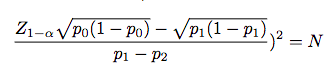
\includegraphics{/users/matthewogle/ds-metrics/pset1/screen.png}

\begin{enumerate}
\def\labelenumi{(\alph{enumi})}
\setcounter{enumi}{5}
\item
\end{enumerate}

Using the rejection region from d)

\[
\sum_{k = c_b}^{n}\begin{pmatrix} n \\ k \end{pmatrix}p_0^k
(1-p_0)^{n-k} \leq \alpha
\]

We need to minimize N number of test kits such that

\[
\sum_{k = c_b}^{n}\begin{pmatrix} n \\ k \end{pmatrix}p_1^k
(1-p_1)^{n-k} \leq \beta
\]

\begin{enumerate}
\def\labelenumi{(\alph{enumi})}
\setcounter{enumi}{6}
\item
\end{enumerate}

\begin{Shaded}
\begin{Highlighting}[]
\NormalTok{N <-}\StringTok{ }\DecValTok{1}\OperatorTok{:}\DecValTok{1000}
\NormalTok{p0 =}\StringTok{ }\KeywordTok{c}\NormalTok{(}\FloatTok{0.001}\NormalTok{,}\FloatTok{0.001}\NormalTok{,}\FloatTok{0.001}\NormalTok{,}\FloatTok{0.05}\NormalTok{,}\FloatTok{0.05}\NormalTok{,}\FloatTok{0.05}\NormalTok{,}\FloatTok{0.001}\NormalTok{,}\FloatTok{0.001}\NormalTok{,}\FloatTok{0.001}\NormalTok{,}\FloatTok{0.05}\NormalTok{,}\FloatTok{0.05}\NormalTok{,}\FloatTok{0.05}\NormalTok{)}
\NormalTok{p1 =}\StringTok{ }\KeywordTok{c}\NormalTok{(}\FloatTok{0.1}\NormalTok{, }\FloatTok{0.15}\NormalTok{, }\FloatTok{0.2}\NormalTok{,}\FloatTok{0.1}\NormalTok{,}\FloatTok{0.15}\NormalTok{,}\FloatTok{0.2}\NormalTok{,}\FloatTok{0.1}\NormalTok{,}\FloatTok{0.15}\NormalTok{,}\FloatTok{0.2}\NormalTok{,}\FloatTok{0.1}\NormalTok{,}\FloatTok{0.15}\NormalTok{,}\FloatTok{0.2}\NormalTok{)}
\NormalTok{beta =}\StringTok{ }\KeywordTok{c}\NormalTok{(}\FloatTok{0.1}\NormalTok{,}\FloatTok{0.1}\NormalTok{,}\FloatTok{0.1}\NormalTok{,}\FloatTok{0.1}\NormalTok{,}\FloatTok{0.1}\NormalTok{,}\FloatTok{0.1}\NormalTok{,}\FloatTok{0.2}\NormalTok{,}\FloatTok{0.2}\NormalTok{,}\FloatTok{0.2}\NormalTok{,}\FloatTok{0.2}\NormalTok{,}\FloatTok{0.2}\NormalTok{,}\FloatTok{0.2}\NormalTok{)}

\CommentTok{# MC model for generating the number of test kits needed }
\CommentTok{## given certain permutations}
\NormalTok{g_mc_model =}\StringTok{ }\ControlFlowTok{function}\NormalTok{(alpha, beta, p0, p1) \{}
  \CommentTok{# defining the replication function with a random sample }
  \CommentTok{# also ensuring that it has a bernoulli distribution}
\NormalTok{  r_sample <-}\StringTok{ }\KeywordTok{replicate}\NormalTok{(}\DecValTok{10000}\NormalTok{, }\KeywordTok{mean}\NormalTok{(}\KeywordTok{rbinom}\NormalTok{(N, }\DecValTok{1}\NormalTok{, p0)))}
  \CommentTok{# Evaluating the test statistic critical value}
\NormalTok{  mean <-}\StringTok{ }\KeywordTok{mean}\NormalTok{(r_sample)}
\NormalTok{  sd <-}\StringTok{ }\KeywordTok{sd}\NormalTok{(r_sample)}
\NormalTok{  critv <-}\StringTok{ }\KeywordTok{qnorm}\NormalTok{(}\DecValTok{1}\OperatorTok{-}\NormalTok{alpha, mean, sd)}
\NormalTok{  p1Beta <-}\StringTok{ }\KeywordTok{pnorm}\NormalTok{(critv, p1, }\KeywordTok{sqrt}\NormalTok{(p1}\OperatorTok{*}\NormalTok{(}\DecValTok{1}\OperatorTok{-}\NormalTok{p1)}\OperatorTok{/}\NormalTok{N)) }
\NormalTok{  result <-}\StringTok{ }\KeywordTok{min}\NormalTok{(}\KeywordTok{which}\NormalTok{(p1Beta }\OperatorTok{<=}\StringTok{ }\NormalTok{beta)) }
  \KeywordTok{return}\NormalTok{(result)}
\NormalTok{\}}

\ControlFlowTok{for}\NormalTok{ (i }\ControlFlowTok{in} \DecValTok{1}\OperatorTok{:}\DecValTok{12}\NormalTok{) \{}
  \KeywordTok{print}\NormalTok{(}\KeywordTok{g_mc_model}\NormalTok{(}\FloatTok{0.05}\NormalTok{, beta[i], p0[i], p1[i])) }
\NormalTok{  \}}
\end{Highlighting}
\end{Shaded}

\begin{verbatim}
## [1] 16
## [1] 10
## [1] 7
## [1] 100
## [1] 27
## [1] 14
## [1] 7
## [1] 5
## [1] 3
## [1] 43
## [1] 12
## [1] 6
\end{verbatim}

\begin{enumerate}
\def\labelenumi{(\alph{enumi})}
\setcounter{enumi}{7}
\item
\end{enumerate}

\begin{Shaded}
\begin{Highlighting}[]
\CommentTok{#let n := number of test kits purchase}
\CommentTok{# in particular, the number of test kits determines the sample size}
\CommentTok{# we will use the smallest n that satisfies alpha < 0.05 and beta < 0.1 (or 0.2 depending on the question)}
\CommentTok{# starting from n = 1.}

\CommentTok{#function binomial probability}
\CommentTok{# pbinom(infected, n, p0)}
\CommentTok{# pbinom is giving me issues}
\NormalTok{p_atleast_m <-}\StringTok{ }\ControlFlowTok{function}\NormalTok{(m, n, p0) \{}
\NormalTok{    prob <-}\StringTok{ }\DecValTok{0}
    \ControlFlowTok{for}\NormalTok{ (j }\ControlFlowTok{in}\NormalTok{ m}\OperatorTok{:}\NormalTok{n) \{}
\NormalTok{        prob <-}\StringTok{ }\NormalTok{prob }\OperatorTok{+}\StringTok{ }\NormalTok{(}\KeywordTok{choose}\NormalTok{(n, j) }\OperatorTok{*}\StringTok{ }\NormalTok{(p0 }\OperatorTok{^}\StringTok{ }\NormalTok{j) }\OperatorTok{*}\StringTok{ }\NormalTok{((}\DecValTok{1} \OperatorTok{-}\StringTok{ }\NormalTok{p0) }\OperatorTok{^}\StringTok{ }\NormalTok{(n }\OperatorTok{-}\StringTok{ }\NormalTok{j)))}
\NormalTok{    \}}
    \KeywordTok{return}\NormalTok{(prob)}
\NormalTok{\}}

\NormalTok{simulation <-}\StringTok{ }\ControlFlowTok{function}\NormalTok{(p0, p1, beta, alpha) \{}
    \CommentTok{#start from n = 1}
\NormalTok{    n =}\StringTok{ }\DecValTok{1}
    \ControlFlowTok{while}\NormalTok{ (}\OtherTok{TRUE}\NormalTok{) \{}
        \CommentTok{#   determine the threshold to reject null}
        \CommentTok{#   threshold is determined by j < n }
        \CommentTok{#   such that the probability of observing }
        \CommentTok{#   at most j infected < alpha}
        \ControlFlowTok{for}\NormalTok{ (thres }\ControlFlowTok{in} \DecValTok{0}\OperatorTok{:}\NormalTok{n) \{}
            \ControlFlowTok{if}\NormalTok{ (}\KeywordTok{p_atleast_m}\NormalTok{(thres, n, p0) }\OperatorTok{>}\StringTok{ }\NormalTok{alpha)\{}
                \ControlFlowTok{next}
\NormalTok{            \} }\ControlFlowTok{else}\NormalTok{ \{}
                \ControlFlowTok{break}
\NormalTok{            \}}
\NormalTok{        \}}
\NormalTok{        threshold <-}\StringTok{ }\NormalTok{thres }\OperatorTok{-}\StringTok{ }\DecValTok{1}
        
        \CommentTok{#run the simulation 1000 times for sample size n}
\NormalTok{        infected <-}\StringTok{ }\KeywordTok{c}\NormalTok{()}
        \ControlFlowTok{for}\NormalTok{ (i }\ControlFlowTok{in} \DecValTok{1}\OperatorTok{:}\DecValTok{1000}\NormalTok{) \{}
\NormalTok{            samp <-}\StringTok{ }\KeywordTok{rbinom}\NormalTok{(n, }\DecValTok{1}\NormalTok{, p1)}
            \ControlFlowTok{if}\NormalTok{ (}\KeywordTok{sum}\NormalTok{(samp) }\OperatorTok{>}\StringTok{ }\NormalTok{threshold) \{}
\NormalTok{                infected <-}\StringTok{ }\KeywordTok{c}\NormalTok{(infected, }\DecValTok{1}\NormalTok{)}
\NormalTok{            \} }\ControlFlowTok{else}\NormalTok{ \{}
\NormalTok{                infected <-}\StringTok{ }\KeywordTok{c}\NormalTok{(infected, }\DecValTok{0}\NormalTok{)}
\NormalTok{            \}}
\NormalTok{        \}}
        
        \CommentTok{#type 2 error is bounded by beta}
        \CommentTok{# thus if we reject the null better than 1-beta }
        \CommentTok{# then we are done}
        \ControlFlowTok{if}\NormalTok{ (}\KeywordTok{sum}\NormalTok{(infected) }\OperatorTok{/}\StringTok{ }\DecValTok{1000} \OperatorTok{>=}\StringTok{ }\DecValTok{1} \OperatorTok{-}\StringTok{ }\NormalTok{beta) \{}
            \KeywordTok{print}\NormalTok{(}\KeywordTok{c}\NormalTok{(threshold, n))}
            \KeywordTok{return}\NormalTok{ (n)}
\NormalTok{        \} }\ControlFlowTok{else}\NormalTok{ \{}
\NormalTok{            n <-}\StringTok{ }\NormalTok{n }\OperatorTok{+}\StringTok{ }\DecValTok{1}
\NormalTok{        \}}
\NormalTok{    \}}
\NormalTok{\}}
\end{Highlighting}
\end{Shaded}

\begin{Shaded}
\begin{Highlighting}[]
\CommentTok{## Simulation results }
\ControlFlowTok{for}\NormalTok{ (i }\ControlFlowTok{in} \DecValTok{1}\OperatorTok{:}\DecValTok{12}\NormalTok{) \{}
    \KeywordTok{print}\NormalTok{(}\KeywordTok{simulation}\NormalTok{(p0[i], p1[i], beta[i], }\FloatTok{0.05}\NormalTok{))}
\NormalTok{\}}
\end{Highlighting}
\end{Shaded}

Results for e:

\begin{enumerate}
\def\labelenumi{\arabic{enumi})}
\item
  24
\item
  15
\item
  10
\item
  17
\item
  231
\item
  7
\item
  77
\item
  4
\item
  37
\item
  16
\item
  11
\item
  7
\end{enumerate}

Results for f:

\begin{enumerate}
\def\labelenumi{\arabic{enumi})}
\item
  22
\item
  15
\item
  11
\item
  226
\item
  76
\item
  39
\item
  16
\item
  11
\item
  8
\item
  154
\item
  52
\item
  27
\end{enumerate}

Note we also collaborated with Zach Yung, Dila Sasmaz, Benamin Jacobs,
Anahita Gogia, Armand Dang, and Rahma Safraoui on this question. We
talked through the theory behind the question together.

\end{document}
